\documentclass{beamer}
\usetheme{CambridgeUS}
\title{Assignment 9}
\graphicspath{{images/}}
\author{Abhishek Kumar}

\institute{IIT Hyderabad}

\date{28May,2022}
\newcommand{\Int}{\int\limits}


\begin{document}
	\begin{frame}
		\titlepage
	\end{frame}
	\begin{frame}{Outline}
		\tableofcontents
	\end{frame}
	\section{Question}
	\begin{frame}{Question Statement}
		
		\textbf{Question:}The joint p.d.f of $X$ and $Y$ is given by:  
		\begin{align}
			f_X_Y(x,y) = \left\{ \begin{array}{ll} 2(1-x) \quad 0 \leq x \leq 1,0 \leq y \leq 1 \\ 0 \quad \text{else} \end{array} \right. 
		\end{align}
		Find the probability density function of z=xy
	\end{frame}
	\section{Solution}
	\begin{frame}{Solution}
		\textbf{Solution:}
		f denotes p.d.f. and F denotes c.d.f.
		\begin{alertblock}{Approach}
			first we will find c.d.f. of z=xy then will differentiate it to get its p.d.f.
		\end{alertblock}
		\begin{align}
			&F_Z(z)=P(Z \leq z)\\
			&F_Z(z)=1 ,z>1\\
			&f_Z(z)=0 ,z>1
		\end{align}
	\end{frame}
	\begin{frame}
		\begin{align}
			&F_Z(z)=\Int_{x=0}^{x=z} \Int_{y=0}^{y=1}f_X_Y(x,y) \,dx\,dy+\Int_{x=z}^{x=1} \Int_{y=0}^{y=z/x}f_X_Y(x,y) \,dx\,dy,0<z\leq1\\
			&\Rightarrow F_Z(z)=\Int_{x=0}^{x=z} \Int_{y=0}^{y=1}2(1-x) \,dx\,dy+\Int_{x=z}^{x=1} \Int_{y=1}^{y=z/x}2(1-x) \,dx\,dy\\
			&\Rightarrow F_Z(z)=2z-z^{2}-2z\log_ez-2z+2z^{2}\\
			&\Rightarrow F_Z(z)=z^{2}-2z\log_ez\\
			&f_Z(z)=2z-2-2\log_ez
		\end{align}
		
	\end{frame}
	\begin{frame}
		\begin{alertblock}{Answer}
			Joint p.d.f. of $z=xy$ is as follows:
			\begin{align}
				f_Z(z) = \left\{ \begin{array}{ll} 2z-2-2\log_ez \quad ,0<z\leq1\\ 0 ,\quad \text{$z>1$} \end{array} \right. 
			\end{align}  
		\end{alertblock}
		\begin{graphics}
			\centering
			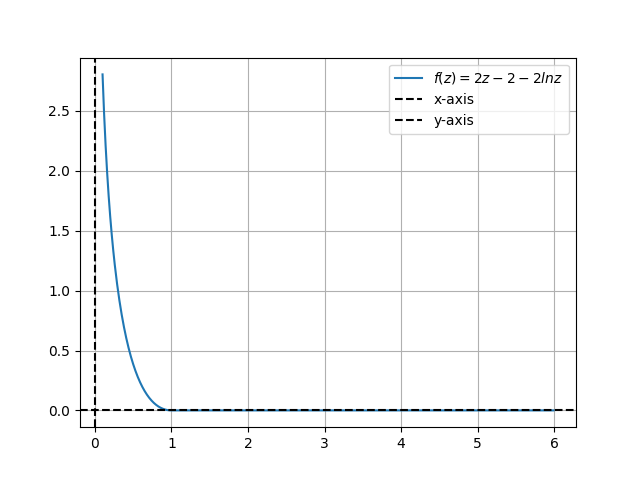
\includegraphics[scale=0.5]{Figure_pdf.png}
			\label{fig-1}
		\end{graphics}
	\end{frame}
	
\end{document}